\documentclass{article}

\usepackage{graphicx}
\usepackage{tikz}
\usepackage{tikzsymbols}
\usetikzlibrary{calc,patterns,shapes.geometric}
\pagestyle{empty}
\usepackage[margin=0pt]{geometry}
\geometry{papersize={14in,12in}}

\def\centerarc[#1](#2)(#3:#4:#5){\draw[#1] ($(#2)+({#5*cos(#3)},{#5*sin(#3)})$) arc (#3:#4:#5);}

\begin{document}
	\begin{figure}
		\centering
		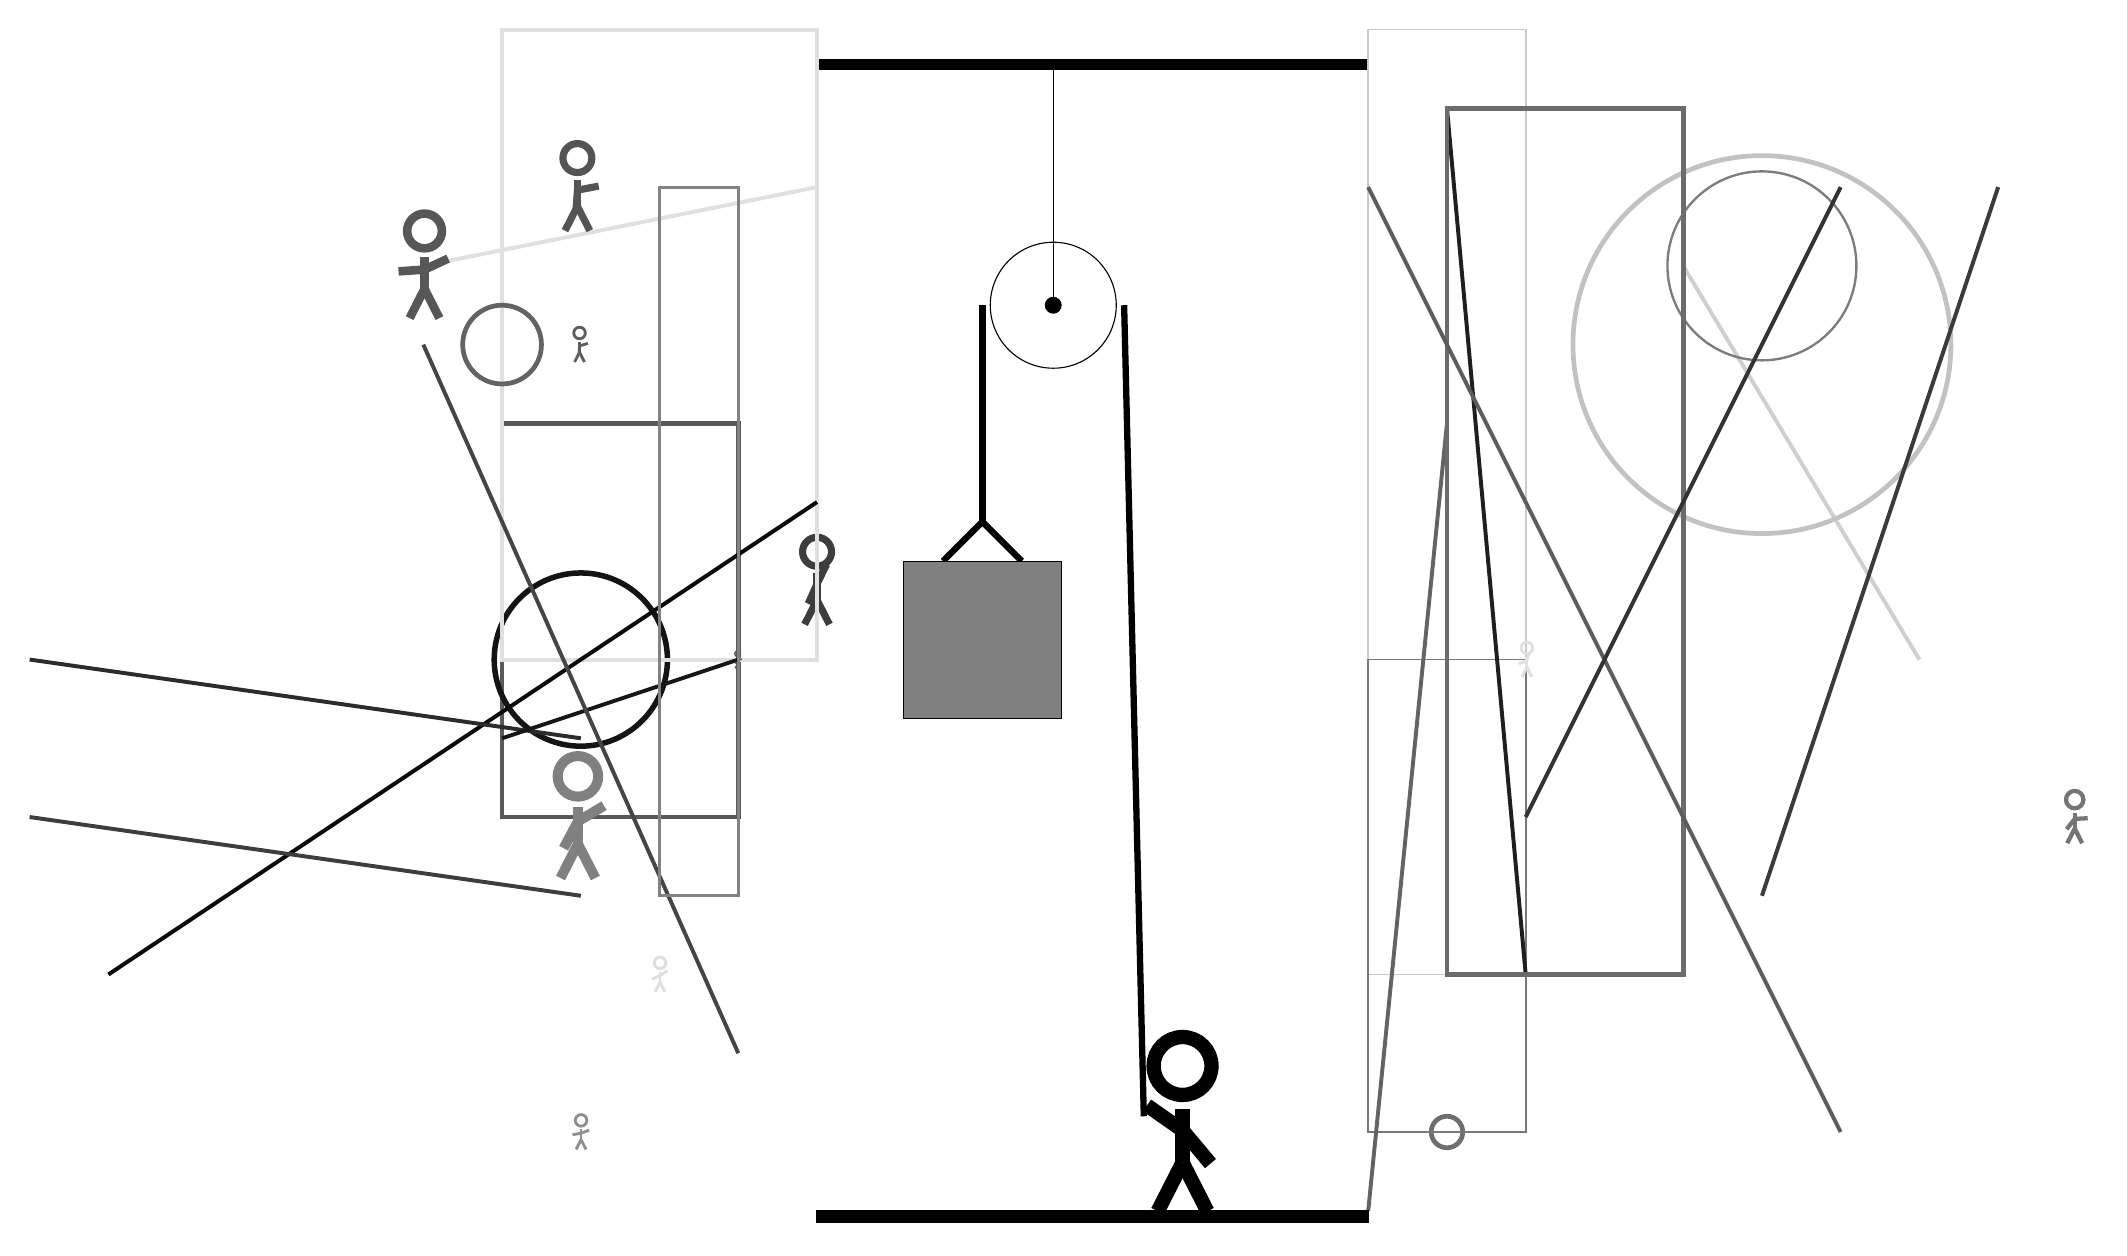
\begin{tikzpicture}
			%%%%% START %%%%%
			
			\draw[fill=black] (-2, 11.5) rectangle (5, 11.625);
			
			\draw (1, 8.5) circle (0.8);
			\draw[fill=black] (1, 8.5) circle (0.1);
			\draw (1, 11.5) -- (1, 8.5);
			
			\draw [line width=0.6mm, color=black!57](6, -2) circle (0.2);
			
			\node[line width=0.5mm, color=black!76] at (-2, 5) {\Strichmaxerl[5][66][64]};
			\draw[line width=0.5mm, color=black!19](9, 9) -- (12, 4);
			\draw[line width=0.2mm, color=black!21] (5, 12) rectangle (7, 0);
			\draw[line width=0.6mm, color=black!65] (-3, 2) rectangle (-6, 7);
			\draw [line width=0.3mm, color=black!51](10, 9) circle (1.2);
			
			\draw [line width=0.7mm, color=black!92](-5, 4) circle (1.1);
			\node[line width=0.2mm, color=black!63] at (-5, 8) {\Strichmaxerl[2][87][16]};
			\draw[line width=0.5mm, color=black!12] (-2, 12) rectangle (-6, 4);
			\draw[line width=0.2mm, color=black!53] (5, 4) rectangle (7, -2);
			
			\draw[line width=0.5mm, color=black!12](-2, 10) -- (-7, 9);
			\draw[line width=0.5mm, color=black!96](-2, 6) -- (-11, 0);
			\draw[line width=0.5mm, color=black!61](6, 7) -- (5, -3);
			\draw[line width=0.5mm, color=black!88](6, 11) -- (7, 0);
			\node[line width=0.5mm, color=black!12] at (7, 4) {\Strichmaxerl[2][20][75]};
			\draw[line width=0.5mm, color=black!83](-5, 3) -- (-12, 4);
			\draw [line width=0.6mm, color=black!24](10, 8) circle (2.4);
			\node[line width=0.3mm, color=black!67] at (-5, 10) {\Strichmaxerl[5][86][11]};
			\node[line width=0.5mm, color=black!66] at (-3, 4) {\Strichmaxerl[1][63][13]};
			\draw[line width=0.5mm, color=black!91](-6, 3) -- (-3, 4);
			\node[line width=0.7mm, color=black!44] at (-5, -2) {\Strichmaxerl[2][10][21]};
			\draw [line width=0.6mm, color=black!61](-6, 8) circle (0.5);
			\draw[line width=0.5mm, color=black!73](-3, -1) -- (-7, 8);
			\draw[line width=0.5mm, color=black!77](10, 1) -- (13, 10);
			\draw[line width=0.6mm, color=black!58] (6, 0) rectangle (9, 11);
			\node[line width=0.2mm, color=black!54] at (14, 2) {\Strichmaxerl[3][52][3]};
			\draw[line width=0.5mm, color=black!64](5, 10) -- (11, -2);
			\draw[line width=0.5mm, color=black!80](7, 2) -- (11, 10);
			\node[line width=0.2mm, color=black!13] at (-4, 0) {\Strichmaxerl[2][22][35]};
			
			\node[line width=0.5mm, color=black!66] at (-7, 9) {\Strichmaxerl[6][4][25]};
			\draw[line width=0.5mm, color=black!76](-5, 1) -- (-12, 2);
			
			\draw[line width=0.4mm, color=black!49] (-4, 10) rectangle (-3, 1);
			\node[line width=0.3mm, color=black!50] at (-5, 2) {\Strichmaxerl[7][62][31]};
			
			
			\draw[line width=0.8mm] (-0.4, 5.25) -- (0.1, 5.75) -- (0.6, 5.25);
			\draw[fill=black!50] (-0.9, 5.25) rectangle (1.1, 3.25);
			
			\draw[line width=0.8mm] (0.1, 8.5) -- (0.1, 5.75);
			\centerarc[line width=0.8mm](1, 8.5)(0:180:0.9);
			\draw[line width=0.8mm](1.9, 8.5) -- (2.15, -1.8);
			
			\node at (2.6, -1.9) {\Strichmaxerl[10][-35][-50]};
			
			\draw[fill=black] (-2, -3) rectangle (5, -3.15);
			
			%%%%% END %%%%%
		\end{tikzpicture}
	\end{figure}	
\end{document}